\documentclass{article}[10 pt]

\usepackage{amssymb}
\usepackage{amsthm}
\usepackage{amsmath}
\usepackage{multicol}
\usepackage{mathrsfs}
\usepackage{graphicx}

\setlength{\oddsidemargin}{0in} \setlength{\evensidemargin}{0in}
\setlength{\textwidth}{6in}
\setlength{\unitlength}{1in}

\linespread{1.5}

\newcommand{\ds}{\displaystyle}
\newcommand{\al}{\aleph_0}
\newcommand{\vs}{\vspace{0.1in}}

\title{The Bitcoin Bridge}

\date{December 1, 2016}

\author{Mitch Lowry}

\begin{document}

\maketitle

This project is a careful, organized attempt at implementing, discussing,
and evaluating different econometric models in the context of explaining the
price formation of Bitcoin. It is important to note here that this project
does not necessarily strive to create a way to predict Bitcoin prices. I
will give an introduction explaining important background information about
Bitcoin, provide the most comprehensive literature review of work done in
any Bitcoin paper, carefully explain the assumptions and limitations of multiple 
regression, the vector auto-regression model, structural equation models, 
and some models for economic bubbles, and investigate whether the use of the 
Ripple payment protocol system has influenced the price of Bitcoin. I review
the literature of Bitcoin pricing and hope to incorporate ideas and data from many
papers so as to create and evaluate a $VAR$ model from an econometrically
sound perspective by considering all of the variables from the onset, and I
also hope to incorporate new, more innovative measures of investor interest
in Bitcoin into a model used to detect multiple bubbles in the Bitcoin price time-series data.

\vs

\textbf{1 Introduction}

\vs

Since the introduction of the Bitcoin by Satoshi Nakamoto on January $3$,
$2009$, an unforeseen number of cryptocurrencies have been created, many of
which are based heavily on Bitcoin. This strange math based phenomenon of
the cryptocurrency piques much debate and interest among economists. Not
surprisingly, most economic research on cryptocurrencies is devoted to the
most highly publicized and valued of cryptocurrencies, Bitcoin; however,
there is a relatively new currency that could significantly impact the
cryptocurrency market and international business. This currency is Ripple’s
XRP. The XRP’s most important role is to act as a bridge currency within
Ripple’s free, open source payment protocol. This payment protocol allows
parties from any part of the globe to perform transactions between any fiat
currencies, commodities, cryptocurrencies, or other stores of value in as
little as five seconds with little to no transaction fees.

\vs

There are many large questions to be tackled about the impact of Ripple on
the global economy; however, the objective of this study is to tackle a
somewhat complex one. I would like to determine whether or not usage of
Ripple has affected the price of the Bitcoin. The rational of this
possibility stems from my belief that the Ripple payment protocol could have
a positive influence on the demand of Bitcoins by making transactions with
Bitcoins safer. Specific details about this will be covered in the
conceptual framework section.

\vs

This paper uses much of the discussion of the fundamental concepts of
Bitcoin described in Fantazzini ($2016$), and also includes some other
information. For more detailed descriptions of Bitcoin see Becket et al.
($2013$), Segendorf ($2014$), Dywer ($2014$), Boehme et al. ($2015$),
Bitcoin ($2015$), Velde ($2013$), Lo and Wang ($2014$), Baden and Chen
($2014$), Ali et al. ($2014$), and ECB ($2012$, $2015$).

\vs

\textbf{1.1 How does Bitcoin Work?}

\vs

Bitcoin is a decentralized payment protocol system. It is composed of a
network of many computers that are connected through the internet. Each of
these computers are called nodes (Cocco and Marschesi $2016$).
The Bitcoin payment system is based off of two concepts: (i) digital
signatures and (ii) a cryptographic hash function. The digital signatures
include a public key and a private key. That is, the location of each
Bitcoin address is represented by an alphanumeric key, known as the public
key, and there exists a private key, known only to the owner of that Bitcoin
address that gives one control of the Bitcoins at that location. For any
payment sent from a specific Bitcoin address, that payment must be verified by
the owner of that Bitcoin address by signing the payment with the private
key associated with that address. This means that knowledge of a Bitcoin's
private key means that you own it (or can at least make transactions with
it, which is essentially the same). These signatures allow three important
things for payments: one can verify who the sender was; one cannot deny 
having sent the message; and the message was not altered in transit. These
signatures provide a security as far as transactions go. At every point in
time, there is a public ledger in Bitcoin balance of every Bitcoin address
is given. Additionally, for each transaction there are one or more sending 
addresses, each of which has an associated amount being sent to one or more
receiving addresses, and each of these receiving addresses has an amount
received; note that this information does not include how much was sent from
each sending address to each receiving address. One has the amount total
sent to the receiving addresses and how much each received, but it is frequently 
not possible to link sending addresses to receiving addresses.
This ledger is updated about every $10$ minutes in blocks of transactions
(Fantazzini $2016$).

\vs

The cryptographic function (in the case of Bitcoin, this is the secure hash
algorithm SHA-256 / type Secure Hash Algorithm SHA-2 (see Dang $2002$ for
details)) is used in conjunction with past transaction history to verify the transactions
in the new block. After the check of a transaction is made through digital
signatures and assuring there is enough money for the transaction,
validation nodes compete to record the transaction into the new Blockchain.
In this way, all transactions since the previous block are recorded by
different network members. In this way, the work is distributed. 
Once this is done, the new block is put into the
hash function and we receive a hash called a digest. This digest is used
with some given one-time use alphanumeric code (nounce), and these two are
used in the second hash function to create a hash for the new block. This is
a computationally heavy task because one must find some random nounce such
that the hash of the new block has some specific number of initial zeros
(Cocca and Merchesi $2016$). Once a node, say node $A$, has found a correct 
nounce, node $A$ tells this nounce to everyone else on the network, who are 
called validation nodes; the validation nodes to see if the nounce works; and 
the new block chain is recorded and node $A$ is given a reward. 
(Cocco and Merchesi $2016$). This reward is in the form of new Bitcoins and 
some voluntary contributions (Fantazzini $2016$).  

\vs

\textbf{2 Literature Review}

\vs

\textbf{2.1 Time-Series Bitcoin Pricing Models}

\vs

Upon reviewing the literature, I came across a literature review published
in May of $2014$ by Ciaian et al. ($2014$), and another literature review
published in $2016$ (Fantazzini et al. $2016$). I review many of the papers
used in these literature reviews and provide a bit more detail. All of the
discussed paper make use of the plentiful amount of time-series data
available about the Bitcoin network. I have also
included papers not included in these literary analyses. In the previous
literature there are quite a few factors that have been identified as
important for determining the price of Bitcoin: ($i$) interacting between
BitCoin demand and supply (Buchholz et al. $2012$; Ciaian et al $2014$;
Kancs et al. $2015$);
($ii$) global financial indicators (van Wijk $2013$; Bouoiyour $2015$); ($iii$)
attractiveness for investors (Kristoufek $2013$; MacDonell $2014$; Ciaian et
al $2014$; Kancs et al $2015$; Bouoiyour $2015$); and ($iv$) and information
related to the creation of Bitcoins (Cocco and Marchesi $2016$; Garcia et
al. $2014$).

\vs

Buchholz et al. ($2012$) use VAR modeling to determine the price of
Bitcoins. The study concludes that the interaction between Bitcoin supply
and demand is a major determinant of Bitcoin prices. These results are
consistent with the results of Ciaian et al. ($2014$) that the
day lag of Bitcoin prices in US dollars, the four day lag of total Bitcoins
that have been mined, and the one and two day lags of Bitcoin days
destroyed. Krancs et al. ($2015$) also find that the lag of Bitcoin prices
is important. Kristoufek ($2013$), however, explains that the price formation
of Bitcoin cannot be explained by standard economic theories because
supply-demand fundamentals are absent from Bitcoin markets. He says this for
the following reasons: ($i$), Bitcoin exists independently of any financial
regulatory systems, so the supply of Bitcoin is detached from what is going
on in the economy, and ($ii$) there are no interest rates for
cryptocurrencies, so profits can only be made on price changes. The problem
with Kristoufek's model and explanation
is that only bivariate VAR for the weekly log-returns of Bitcoin prices and
is employed, and other variables
that have been found important in more contemporary literature were not
considered in conjunction with these other variables, which could result in
omitted variable bias, and, thus, model misspecification. Kristoufek
($2013$) uses a bivariate Vector Error Correction (VEC) model in conjunction
with his bivariate VAR. This paper was
interesting in that it used normalized daily Google search data to gauge
the interest in Bitcoin, and it uses the daily views of the Bitcoin
wikipedia page an alternate proxy. This was the first paper to include
the speculative nature of Bitcoin. He created a positive feedback variable
and a negative feedback variable and found a
bidirectional relationship between search queries and prices viceversa.
Again, this should be taken with a grain of salt, but including this
feedback idea into models that consider more regressors is a good idea. The
feedback loops used by Kristofek ($2013$) are discussed in Section 2.2.

\vs

Van Wijk ($2013$) stresses that since Bitcoin is a fiat currency, the only
reason Bitcoin has value is because investors and other buying agents
believe that Bitcoins will retain their value. He claims that general
economic indicators are good indicators of whether or not Bitcoin will
retain its value, so he performs Ordinary Least Squares (OLS) on Bitcoin
prices with such
indicators and then applies an error correction model to get long term
relationships because performing OLS on differenced variables results in
loss of long run effects in the outcome of the analysis. Van Wijk ($2013$) found that
in the short run the only variable that had a significant influence on the
value of Bitcoin was the closing value of the Dow Jones index (positive
influence) but that there were insignificant variables, namely the closing
value of the Nikkei $225$ (negative influence), the euro-dollar exchange
rate (positive influence) and the yen-dollar exchange rate (positive
influence), with large coefficients that may explain some of the variation
in Bitcoin. Whether this is a legitimate claim or he is just trying to make
himself look better is up for debate. In the long run he found that the
following variables were important for determining the price of Bitcoin:
($i$) Dow Jones index (positive influence), ($ii$) the euro-dollar exchange
rate (negative influence), and ($iii$) the jen-dollar exchange rate
(negative influence). Dimitrova ($2005$) claims that there could be a
negative relationship between Bitcoin prices and financial indicators.
Dimitrova ($2005$) says that if stock prices fall, then foreign investors
may decrease their stock with BitCoin; however, what Dimitrova does not
account for here is that a decline in the price of some stock may also be a
signal to purchase that stock if one does not currently hold any of it (or
even if they do). Ciaian et al. ($2014$) and MacDonell ($2014$) find no such
relationships between Bitcoin prices and macroeconomic indicators.

\vs

MacDonell ($2014$) used log-periodic power law (LPPL) modeling in an attempt to
make a model that can predict crashes in Bitcoin prices. The motivation from
this clearly stems from the major Bitcoin bubble of $2013$. Of the variables
MacDonell tested, only the CBOE Volatility Index was found to be
significant, which implies that only investor behavior matters for
determining the prices of Bitcoins. This is likely due to the fact that
MacDonell used news mentions as a proxy for consumer participation. This
does not seem like a good enough proxy, and so the regression would not
really parallel consumer participation. Both Kristoufek ($2013$) and Ciaian
($2014$) found that indicators of the Bitcoin supply and demand were
significant in determining the price of Bitcoin in the short run and in the
long run. They used a somewhat more reasonable proxy for attractiveness for
investors, the volume of daily BitCoin views on Wikipedia. According to
Kristoufek ($2013$) this proxy is a good indicator of how interested
investors are in Bitcoin. Fry ($2014$) and Fry ($2015$) continue improving
and using the LPPL model and confirm that there was a bubble in December of
$2013$ before the large price crash. They also found that the long term
fundamental value of Bitcoin in zero, and that the bubble component of the
model accounts for 48.7 percent of all prices. Work has been done to
create tests for mulitple bubbles by using a movingn time window (Phillips
and Yu $2011$; Phillips et al. $2011$; and Phillips et al. $2015$). This
model is called the generalized-supremum ADF test (GSADF). Malhotra and
Maloo ($2014$) implement the ADF and find bubble like behavior from August -
October $2012$ and Novemeber $2013$ - February $2014$. These bubble models
demonstrate the importance of including speculative variables in regressions
involving Bitcoin prices. These bubble models are discussed in section 

\vs

Glaser et al. ($2014$) used a vector auto-regressive model with lagged
effects and GARCH effects. They found, unlike anyone before them, that Bitcoin
attractiveness and Bitcoin supply and demand were both important regressors.
This paper follows the lead of Kristoufek ($2013$) and also uses the daily views on
the English Bitcoin Wikipedia as a proxy for user interest.
This paper was also helpful for future modeling in that dummy variables for
$24$ events gathered from $https://en.bitcoin.it/wiki/History$. These events
were either significant positive or negative events. This work was done
using a four-variate VAR(1) model with first-differenced data from January
$2009$ to October $2013$. This model, like that of Kristoufek, finds a couple of positive
feedback loops. The first one is that increased Bitcoin popularity, leads to
more searches of Bitcoin, which is related to more social media posts about
Bitcoin, which causes more people to buy Bitcoin, which increases Bitcoin
prices. Secondly, after users get information about Bitcoin, they download
the client, and the increase in the number of users, which drives up prices because
supply is deterministic.

\vs

Garcia et al ($2014$) extend this research on speculation by using different
variables. Garcia uses the following variables in a 4-variables in a VAR(1)
model, which shows that there is a negative relationship between searches and
prices:

\begin{itemize}
    \item number of new Bitcoin users adopting the currency at time $t$,
        which is proxied by the number of downloads of Bitcoin software
        client;
    \item bitcoin price in USD, EUR, and CNY;
    \item information search proxied by normalized daily Google search data
        (and uses daily views of the Bitcoin wikipedia as a robustness
        check);
    \item information sharing (or online word-of-mouth communication)
        proxied by the daily number of tweets about Bitcoin $B_1$ per
        million twitter messages. Data was taken from http://topsy.com, and
        the following terms were used to find tweets about Bitcoin: 'BTC',
        '#BTC', 'bitcoin', or '#bitcoin'.
    \item valence (some measure of general positiveness of twitter feeds)
    \item other thingy bob maybe.
\end{itemize}


This model, like that of Kristoufek, finds a couple of positive
feedback loops. The first one is that increased Bitcoin popularity, leads to
more searches of Bitcoin, which is related to more social media posts about
Bitcoin, which causes more people to buy Bitcoin, which increases Bitcoin
prices. Secondly, after users get information about Bitcoin, they download
the client, and the increase in the number of users, which drives up prices because
supply is deterministic.

\vs

A couple of econometricians (Bouoiyour and Selmi $2015$; ) talk about their
model. It is useful because has interpretable long-term affects and
short-term effects. The model also reaches an equilibrium, and has the
advantage that effects found are interpretable in a meaningful way. They
found blah blah blahh

\vs

\textbf{2.2 Bitcoin Attractiveness to Investors}

\vs

The attractiveness of Bitcoin to investors and to vendors depends on both
the risk and return of buying and performing transactions with Bitcoins.
Vendors accepting Bitcoin may also be worried about the costs of converting
Bitcoins into other currencies because the economies that they function in
do not operate with Bitcoins. One important risk to consider is the security
of Bitcoin exchanges. Since Bitcoin is a digital currency there is a very
real threat of cyber-attacks. In fact, Moore and Christin ($2013$) found
that of the $40$ Bitcoin exchanges that they examined $18$ closed down
because of cyber-attacks in which users information and or Bitcoins were
stolen. Another thing to consider for investors is the cost of finding out
what is worth investing in. Many studies (Gervais, Kaniel, and Mingelgrin
$2001$; Grullon, Kanatas, and Weston $2004$; and Barber and Odean $2008$)
have found that the decisions of new investors may be distorted by the
effect of media attention. This is the rational for the use of news mentions
by MacDonell ($2014$); however, news mentions doesn't seem like good variable
for either an explanatory or a predictive standpoint. These is good and bad
news, and no way from this variable to tell whether the news is good or bad
or even how significant. If one where to have to use one or two measures 
of noise chasing to avoid spurious information and multicolinearity, ones
that capture how the public feels about media or
social media as done in Garcia et al ($2014$) and large positive or negative 
events in the Bitcoin economy. Such events could potentially be covered
by dummy variables.

\vs

Here is will discuss the reasoning behind and the construction of the two
feedback loops used by Kristoufek ($2013$) and it's potential in different 
models or something. Especially in a regression, and what the other
literature tells us about these affects, much just pulling from the
literature. I will also discuss potential variable to use for these feedback
loops.

\vs

Another variable that has been found significant by some of these studies is 
Data on the daily Bitcoin days destroyed,
$b_dd$ is used as a proxy for the velocity of Bitcoins. This is a pretty
good indicator of Bitcoin hoarding. This measure is added to after each
transaction during the day. The amount added to the measure for each
transaction on a given day is equal to the sum of the days since each
Bitcoin was spent for each Bitcoin. That is, change in the rate of change of
$b_dd$ while adjusting for the total number of Bitcoins in circulation
seems like a good measurement of changes in hording. In the short-run large
decreases in the Bitcoin days destroyed may signal that people who has
previously been hoarding are starting to spend their BTCs. If we view people
who have been hoarding for a long time as wise (they have done quite well), 
then a large change in their hoarding behavior may be a sign to start
selling Bitcoin. These people may on average by more informed than all of
the unfortunate people who didn't buy in early or sold out. Since one cannot
link Bitcoin sending addresses to specific Bitcoin receiving addresses on
Bitcoin (which would be a cool way to monitor other buyers), this seems
like a good measurement for seeking information. One important thing to
consider is the 

\vs


\textbf{2.3 Economics of Bitcoin Mining}

\vs

Since BitCoin has no intrinsic value and is a fiat currency, demand for
BitCoins is primarily determined by its expected value in the future, i.e.
people do not want to accept or exchange for BitCoins if they believe the
price of BitCoin is going to be lower when they plan on using said BitCoins.
The supply of BitCoins is determined by the total number of BitCoins in
circulation. BitCoins are generated by BitCoin “miners” who, either
individually or in groups, complete the computationally difficult problem of
finding and adding blocks to the BitCoin block chain, BitCoin’s public
ledger of past transactions. As mentioned in the backgorund, when miners find a block and update the public
ledger, they are given a reward in the form of Bitcoins and voluntary
controbuitions. New BitCoins are generated and given to the miners as
compensation in addition to some donated funds. The hope here was the
donated funds would eventually take over for securing interest in confirming
transactions on the Bitcoin network as the award twindles. The interesting
thing here is that of in the long-run, due to the slowed increase and
stopping in growth that there may be large amounts of inflation. Proponents
counter this by pointing out that Bitcoins are divisible up to 8 decimal
places, and that could even be adjusted.

\vs

The difficulty of finding blocks (Usually measured in some form of
Hashes/Bitcoin) is adjusted every 2016 blocks based on the
total computational power going into mining. This adjustment results in a
steady rate of mining; a new block is added to the ledger every ten minutes.
The reward that miners receive from finding these blocks is halved every
$210000$ blocks, which means over two year periods there is a relatively linear
increase in the number of BitCoins. This decrease in the reward also means
that there is a predefined number of BitCoins in the long-run. This will be
$21$ million BitCoins in $2140$. The process of adding blocks to the ledger
is a way to insure an accurate public ledger, and, thus, is related to the
security of the Bitcoin system (Nakamoto $2008$). One problem here, as
hinted at earlier, is that this decrease in the award for Bitcoin
disincentives miners that are not optimistic about the market.

\vs

Talk about using valence in models, and twitter stuffs.

\vs

\textbf{3 Theory}

\vs

As previously discussed, studies have found the following things to be
important for determining the price of Bitcoin: ($i$) interaction between
Bitcoin demand and supply; ($ii$) global financial indicators; ($iii$)
attractiveness for investors; and ($iv$) drivers related to the nature of
the construction of Bitcoin.

\vs

\textbf{3.1 Supply-demand Theory}

\vs

In the spirit of Ciaian et al. ($2014$) we will also use a modified version
of Barro’s ($1979$) model to discuss the theory of the interaction between
money supply and demand. Firstly, we note that in perfect markets there is
equilibrium between money supply and money demand. The Bitcoin model is
certainly not a perfect market, but there may be a similar relationship here
as with other fiat currencies. For Barro’s model we have the following
equation for the supply of Bitcoins:

\vs

($1$) \begin{center} $M^{S} = P^{B}B$. \end{center}

\vs

In the above equation $M^{S}$ denotes the supply of Bitcoins, $P^{B}$
denotes the price of Bitcoins in US dollars, and $B$ denotes the total
number of Bitcoins. Based on the Fischer equation money demand $M^{D}$ is
dependent on the general price level of goods, $P$, the size of the Bitcoin
economy, $Y$, and the velocity of Bitcoins, $V$. The assumed equation is as
follows:

\vs

($2$) \begin{center} $M^{D} = \dfrac{PY}{V}$. \end{center}

\vs

Using the equations one can derive the following price relationship:

\vs

($3$) \begin{center} $P^{B} = \dfrac{PY}{VB}$. \end{center}

\vs

This equation implies the following things about the price of Bitcoin: ($i$)
Bitcoin prices decrease as the velocity and total stock of Bitcoins
increases, and ($ii$) Bitcoin prices increase as the general price level and
the size of the Bitcoin economy increases. Thus, we can construct some model
of Bitcoin prices by the following:

\vs

($4$) \begin{center} $p_{t}^{B} = \beta_{0} + \beta{1}p_t + \beta_{2}y_t +
    \beta_{3}v_t + \beta_{4}b_t + \epsilon_t$ \end{center}

where each lower case variable is a some measure its corresponding uppercase
variable and $\epsilon_t$ is the error term at time $t$.

\vs

\textbf{3.2 Adding Attractiveness to Investors and Vendors and Macroeconomic
Indicators}

\vs

Those things that should increase the security of using Bitcoin and reduce
transaction costs or potential transaction costs should increase
attractiveness of Bitcoins to both investors and vendors. Theoretically,
this should increase the demand of Bitcoins, thereby, increasing the price
of Bitcoins by a loose interpretation of equation ($3$); however, the
previous literature review demonstrates that this is not necessarily true.
Besides what we have already discussed, one of the largest risks of
investing in and accepting Bitcoins as compensation is the high price
volatility that Bitcoin is plagued with. This volatility may actually
simulate investment, especially when the volatility of the stock market is
especially low due to the allure of the possibility of large returns;
however, there is obviously good reason to shy from investing in things with
such volatility. This high volatility also imposes additional risk on
vendors because vendors who do accept Bitcoins may receive less (or more) money than
they were supposed to receive due to prices changing before they are able to convert their Bitcoins
into whatever currency they would like.

\vs

As previously discussed, a new block is added to the Bitcoin chain block
every ten minutes. This means that the average time that one has to wait in
order to convert their Bitcoins into another currency is five minutes. Due
to the high price volatility of Bitcoin the vendor may receive less money
than they had hoped, will incur transaction fees, and perhaps a little
stress or actual costs from training employees and dealing in Bitcoins. In
enters Ripple. Ripple is a cryptographically secure internet protocol that
is a peer-to-peer payment system. When using Ripple, XRP acts as a bridge
currency so that one Ripple user can pay in the currency of their choice and
the other Ripple user can receive said payment in the currency of their
choice. This is done with phenomenally low transaction fees. The fees are
set to be essentially zero, but not zero so as to protect from adversaries
of Ripple who may try to overload the Ripple ledger by spamming transactions
(Schwartz et al. $2014$). 

\vs

This payment system decreases many of the negative aspects of dealing in
Bitcoins and investing in Bitcoins. For one thing, volatility is much less
of an issue for both investors and vendors. This is because one is able to
use the Bitcoin Bridge (the integration of the Bitcoin network and Ripple)
to more quickly convert Bitcoins into a currency of their preference or to
more quickly liquidate Bitcoin holdings. Ten minutes may be a long time
given the price volatility of Bitcoin, but a matter of seconds is almost a
laughable amount of risk. The Bitcoin Bridge also helps to reduce the risk
associated with using Bitcoin exchanges. People with Ripple wallets need not
ever directly work inside of payment systems specific to Bitcoin, and their
personal information is safer and transactions, more secure. 

\vs

By our previous discussions we expect those macroeconomic indicators that
are positively related to the general price level of good to be positively
related to the price of Bitcoins and those that are negatively related to be
negatively related to the price of Bitcoins.

\vs

Thus, we adjust equation ($4$) as follows to account for the attractiveness
to investors and macroeconomic indicators:

\vs

($5$) \begin{center} $p_{t}^{B} = \beta_{0} + \beta_{1}p_t + \beta_{2}y_t +
    \beta_{3}v_t + \beta_{4}b_t + \Sigma \gamma_{i}a_{i_t} + \Sigma
    \alpha_{j}m_{j_t}  + \epsilon_t$ \end{center}

\vs

where each $a_{i_t}$ is an indicator of Bitcoin's attractiveness to
investors and each $m_{i_t}$ is a macroeconomic indicator.

\vs 

\textbf{3.3: Adding Variables Related to Mining}

\vs



\vs

\textbf{4 Data}

\vs

All data was acquired from \textit{quandl.com}. All data is daily data
ranging from August $5$, $2010$ until October $28$, $2016$. There are
different days missing for each of the variables, so the total number of
observations will depend on the regression. 

\vs

The dependent variable is the
BTC-USD exchange rate, $price_\{ave\}$ in US dollars averaged over all $24$
hours over all Bitcoin markets. 

\vs

Data on the daily Bitcoin days destroyed,
$bcdde$ is used as a proxy for the velocity of Bitcoins. This is a pretty
good indicator of Bitcoin hoarding. This measure is added to after each
transaction during the day. The amount added to the measure for each
transaction on a given day is equal to the sum of the days since each
Bitcoin was spent for each Bitcoin. That is, change in the rate of change of
$bcdde$ while adjusting for the total number of Bitcoins in circulation
seems like a good measurement of changes in hording. In the short-run large
decreases in the Bitcoin days destroyed may signal that people who has
previously been hoarding are starting to spend their BTCs. If we view people
who have been hoarding for a long time as wise (they have done quite well), 
then a large change in their hoarding behavior may be a sign to start
selling Bitcoin. These people may on average by more informed than all of
the unfortunate people who didn't buy in early or sold out. Since one cannot
link Bitcoin sending addresses to specific Bitcoin receiving addresses on
Bitcoin (which would be a cool way to monitor other buyers), this seems
like a good measurement for seeking information.

\vs

Also, as determinants of the Bitcoin economy, the number of Bitcoins in 
circulation, $BTC$_t is used for the supply of Bitcoins at time $t$, 
and the number of unique Bitcoin transactions, $T^d_t$, and the number 
unique Bitcoin accounts, $Num_User$_{day}, used in transactions are used as 
proxies for Bitcoin demand. 

\vs

Additionally, oil prices are a good macroeconomic indicator of the future
price of goods, so the prices of Brent Oil, an international oil company are
used ($brent\_day$). Also, the value of the DOW Jones is used as a price
indicator and an indicator of attractiveness to investors. For the same
reasons, the Euro-USD exchange rate, $usd\_eur$, and the USD-JPY exchange
rate, $usd\_jpy$ are considered for the model.

\vs

Sadly, I could not figure out how to collect data from the Ripple charts API
to find the total number of Ripple accounts over time. This would have
served as a measure for how much Ripple is used. My original hypothesis is
that the actual use of Ripple account, independent of the transactions
performed on said accounts, would influence the price of Bitcoin by
affecting the attractiveness of Bitcoin to investors and vendors. Another
important variable that would have been good for determining the
attractiveness of Bitcoins to investors and vendors would have been data on
the daily Wikipedia hits of Bitcoin, as noted in the literature review.

\vs

I hope also to collect data on valence and tweets. And there is one more
super interesting data set I want to collect.

\vs

\textbf{5 Modeling Considerations}

\vs

Paragraph about models in general

\textbf{5.1 VAR Modeling}

\vs

Talk about the model. What is it? What are the assumptions?

\vs

What is autocorrelation?

\vs

What happens to the model if this is not met?

\vs

What are tests for it? Talk about Durbin-Watson.

\vs

What are fixes for it?

\vs

What is heteroskedasticity?

\vs

What happens to this model if this is not met?

\vs

What are tests for it? 

\vs

What are fixes for it?

\vs

Talk about What happens to the model if this is not met? What are fixes for it?

\vs

What is multi-colinearity?

\vs

What happens to the model if this is not met? What are fixes for it?

\vs

Talk about modeling misspecification. Talk about spurious relationships
caused by non-stationarity. 

\vs

What are tests for non-stationarity? Augemented Dickey-Fuller

\vs

Talk about testing for co-integration

\vs

Talk about model misspecification test - RAMSEY Reset Test

\vs

\textbf{5.2: Bubble Modeling}
\textbf{6: Expectations}

\vs

The expectations of this model specification are hard to determine based on
the lack of data. I estimate, based on the literature, that because of the
inclusion of measures of the supply and demand of Bitcoin, macroeconomic
indicators will mostly not be important in determining the price of Bitcoin.
I believe that the measures of Bitcoin supply and demand play out as
explained in the literature review and conceptual framework. Also, exchange
rates may or may not be significant.

\vs

\textbf{7 Preliminary Analysis}

\vs

Firstly, summary statistics were calculated for all of the initial
variables, and line graphs for all of the data (Appendix A). The descriptive
statistics do not necessarily tell us much; however, the line graphs are
quite useful. Firstly, note that the graphs suggest that we may need to do
a log transformation of the prices for Bitcoin. The graphs also give us some
intuition about the stationarity of the time series, as discussed below.

\textbf{7.1 Handling Stationarity}

\vs

In order to specify a VAR model that is not spurious, we must ensure that
the variables of the model are cointegrated; however, performing tests of
stationarity cannot be performed when there are gaps in the data unless
specialized fixes are performed. Gaps in the data are necessary
consequences of how macroeconomic indicators are recorded. Of the variables
with no gaps, $price\_ave$, $totcoins$, $usd\_jpy$, and $usd\_eur$, all are
non-stationary. The augmented Dickey-Fuller tests were applied to the time
series for the tests (Appendix B). Since it is outside of the scope of this
project to attempt to perform specialized tests for non-stationarity, I
will have to use all of the information that I have. First, we checked to
see if each of $price\_ave$, $totcoins$, $usd\_jpy$, and $usd\_eur$ are
$I$($1$) by performing another Augmented Dickey-Fuller test on the
differenced variables (Appendix B). Indeed, there is evidence that every
variable is stationary. In fact, even at $\alpha = .01$ all models are
stationary all the way up to lag $23$ except for $dif\_totcoins$, which is
stationary up to $17$ lags but still stationary up to $23$ lags at
$\alpha=.05$.

\vs

The Bitcoin algorithm for adjusting the computational difficulty of
algorithms results in a constant increase of Bitcoins, as can been seen by
the line graph of $totcoins$ (Appendix A). Because of this, the variance
may be fairly constant, but the average is not. Thus, we find it likely
that $totcoins$ is of order of integration one, but we may specify some
models in which this is not an assumption. Looking at the line graph for
daily Bitcoin days destroyed during the period in which we are using the
data, the variance appears to be relatively constant, especially when
excluding massive drops in Bitcoin prices and seasonal events like
Christmas, Cyber-Monday, and Black Friday. Due to the relatively large
number of data points, I believe even without adjustment this will result
in the data being stationary. This is consistent with findings of the
velocity of money that suggest a borderline relationship in some tests and
stationarity indeed in others (Aslan and Korap $2007$; and Brand et al.
$2002$). Thus, I believe it to be probable that $bcdde$ is stationary.
Based on the line graphs, $address\_day$ and $trans\_day$ seem to be of
order integration of $I$($1$), especially as of late. This is consistent
with the literature review.

\vs

A recent study by Bacon and Kojima ($2008$) suggests that both oil prices
and the log transformation of oil prices are non-stationary with order
$I$($1$). This suggests that both $brent\_day$ and $ln\_brent\_day$ will be
non-stationary with $I$($1$). Mr. David Alan Dickey himself points out how
obvious it is that the log transformation of the Dow Jones Index is
non-stationary of order one (Dickey, David $2005$) and tests these
hypothesizes. I am unsure about what the literature has to say about the
stationarity of the Dow Jones Index itself. The Dow Jones looks very
clearly like a non-stationary variable with $I$($1$) based on the line
graph, i.e. if one draws a fairly straight, positively sloped line through
the data in the right location, then you can see that the variance of
differences seems to be fairly constant and that the differences are
centered about some mean. Thus, we also assume that $ln_dj_day$ and
$dj_day$ are of order $I$($1$). 

\vs

The stationarity of those log transformed variables for which it was is
possible to perform an Augmented Dickey-Fuller test without transformations
was tested (Appendix B). Indeed, each of the log transformations of
$totcoins$, $usd\_eur$, $usd\_jpy$, and $price\_ave$ are $I$($1$). I am
done with the analysis of stationarity. I will base base modeling off of
the available information, which includes information from the
Dickey-Fuller and the literature about what lags may be important.

\vs

\textbf{6.2 Preliminary Regressions}

\vs

The first two regressions run for price estimation are in Appendix C.
Initially, I attempted to keep in all cointegrated variables and then add
in lags that I thought were important. My initial model failed in every
respect: there was multicolinearity, autocorrelation, heteroskedasticity,
and most importantly, misspecification. The mulicolinarity was clear,
although not tested for; autocorrelation was indicated by failing the
Augmented Durbin Watson test, which is valid for models that have lags of
the dependent variable as independent variables; heteroskedasticity is
indicated by rejecting the null in the Breusch-Pagen test; and both the
failed Durbin Watson test and the failed Ramsey RESET test indicate
misspecifcation of the model. The price of Bitcoin is clearly not linear,
as previously discussed. The autocorrelation and homoskedasticity are also
clear in Figures $30$ and $31$. The model does past the F test, but of all
the variables only the first and second day lags of bitcion price and the
$address_day$ were found to be signficant. 

\vs

In a vain attempt to make the model better, I decided to take out variables
that were causing multicolinearity and that were not that predictive
(Appendix C). The lag of exchange rates make much more sense, and the
number of unique Bitcoin addresses from which purchases were made on any
given day has, without a doubt, a very high correlation to the number of
unique Bitcoin transactions performed on a day. Thus, I decided to keep the
better proxy, the number of unique Bitcoin transactions on a given day. I
believe the number of transactions would be a better proxy unless there
were people spamming the network with very low payments, which would be
financially costly in the Ripple system but especially so in mainstream
Bitcoin exchanges. One can see from Figure $31$ that the model is in no
better shape than its predecessor. The very low p-values for the Durbin
Watson tests suggest the regression is spurious.

\vs

I followed up these regressions by modeling the logarithmic price of
 Bitcoin (Appendix D). 

\vs

\textbf{7 Results of “Best” Models}

\vs

The model found in figure $24$ seems to have been the best model I could
come up with. The model passes specification testing via the Ramsey RESET
test, just barely checks in as having homoskedasticity by the Breusch-Pagen
test, and has such a high probability for the Durbin Watson that it does
not appear to be spurious or have autocorrelation. This should be weighed
carefully because the Breusch-Pagen test only tests for linear
heteroskedasticity. Interestingly, lagged exchange rates are now
considereed important for determining Bitcoin prices. The meaning of the
signs on these coeifficents is up for debate though. 

\vs

If one removes the log of total Bitcoins from the regression because of its
insignifance in determining prices, they will find that the probability of
there being heteroskedasticity increases to the ponit of being signficant at
$\alpha=.05$ (Figure $38$). Also, one should note the extremely high
correlation between the one day lag and the two day lag in Bitcoin prices.
Removing one of these lags results in failing of the Durbin Watson test.   

\vs

\textbf{8 Summary and Implications}

\vs

An interesting result here is that the model goes from being a seeming
pretty good model in terms of explaining having autocorrelation when the
second llag of bitocoin prices is removed. I think this is because it takes
away this sort of idea that Bitcoin investors and potential Bitcoin
investors are not only thinking about what happened when it comes to the
immediate but also to slightly before that when trying to determine what
will happen to the price of Bitcoin. This is because the price volatility
of Bitcoin is phenomenal. Furthermore, these regressions have very large
$R^2$ values, and it should be determined whether or not their residuals
are stationary so as to reduce the possibility that these regressions are
spurious. Similiar to the literature, we found that the demand for Bitcoins
was more important for determining bitcion prices. Indeed, we found that
the supply of Bitcoins was not an important determinant. All results should
be taken lightly because of the possibility of many omitted variables that
could have biased the results.

\vs

\textbf{9 Future Work}

\vs

Future work on this project will involve a more indepth study of solving
endogeniety problems. I could try performing more complex error correction
models within the VAR framework, or more interestingly, work with
simultaneous equations. Either way, I would still like to take another look
at this problem when I have collected data from Ripple and gotten data on
the price volitility of Bitcoin. I would also like to learn how to test for
stationarity when there is gaps in the data. In addition to this, one thing
I am particularly interested in is using machine learning for prediction. 

\newpage

\begin{center}

\textbf{References}

\end{center}

\vspace{5mm}

Aslan, O. and Korap, L. ($2007$). Testing Theory of Money for the Turkish
Economy. \textit{BDDK}
$https://www.bddk.org.tr/WebSitesi/turkce/Raporlar/BDDK_Dergi/4212Makale-5.pdf$

\vs

Bacon, R. and Kojima, M. ($2008$). “Coping with Oil Price Volatility”.
\textit{ESMAP} $05$/$008$
$http://www.esmap.org/sites/esmap.org/files/8142008101202_coping_oil_price.pdf$ 

\vs

Barber, B.M. and T. Odean ($2008$). All That Glitters: The Effect of
Attention and News on the Buying Behavior of Individual and Institutional
Investors.
\textit{Review of Financial Studies}

$21$($2$): $785-818$. 

\vs

Brand, C., Gerdesmeier, and D., Roffia ($2002$). “Estimating the Trend of
M3 Income Velocity Underlying the Reference Value for Monetary Growth.”
\textit{European Central Bank} $3$ $1-61$
https://www.ecb.europa.eu/pub/pdf/scpops/ecbocp3.pdf

\vs

Buchholz, M., Delaney, J., Warren, J. and Parker, J. ($2012$). “Bits and
Bets, Information, Price Volatility, and Demand for Bitcoin.”
\textit{Economics} $312$,
$http://www.Bitcointrading.com/pdf/bitsandbets.pdf$

\vs

David, D. ($2005$). “Stationary Issues in Time Series Modeling”.
\textit{Sugi} $30$: $192-30$.
$http://www2.sas.com/proceedings/sugi30/192-30.pdf$

\vs

Dimitrova, D. ($2005$). The Relationship between Exchange Rates and Stock
Prices; Studied in a Multivariate Model.” \textit{Issues in Political
Economy} $14$: $1-25$.

\vs

Gervais, Simon, Ron Kaniel, and Dan H. Mingelgrin. ($2001$). The
high-volume return

premium. \textit{Journal of Finance} $56$: $877–919$. 

\vs


Grullon, G., Kanatas, G. and Weston, J.P. ($2004$). Advertising, breadth of
ownership, and liquidity.\textit{Review of Financial Studies} 17: 439–61.

\vs

Kristoufek, L. ($2013$). “BitCoin meets Google Trends and Wikipedia:
Quantifying the relationship between phenomena of the Internet era.”
\textit{Scientific Reports} $3$ ($3415$): $1-7$.

\vs

Nakamoto, S. ($2008$). Bitcoin: A Peer-to-Peer Electronic Cash System.
\textit{The Cryptography Mailing List}, $1-9$.

\vs

MacDonell, Alec ($2014$). “Popping the Bitcoin Bubble: An application of
log-periodic power law modeling to digital currency to digital currency.”
\textit{University of Notre Dame}
$http://economics.nd.edu/assets/134206/mac_donell_popping_the_biticoin_bubble_an_application_of_log_periodic_power_law_modeling_to_digital_currency.pdf$

\vs

Moore, T. and N. Christin ($2013$). “Beware the Middleman: Empirical
Analysis of BitCoin-Exchange Risk.” \textit{Financial Cryptography and Data
Security} $7859$: $25-33$.

\vs

Schwartz, D., Youngs, N., and Britto, A. ($2014$), The Ripple Protocol
Concensus Algorithm. \textit{Ripple Labs Inc.}
$https://ripple.com/files/ripple_consensus_whitepaper.pdf$

\newpage

\textbf{Appendix A: Preliminary Analysis}

\vspace{5mm}

\begin{center}

\begin{figure}

\end{figure}

\end{center}\begin{figure}[ht!]

\centering

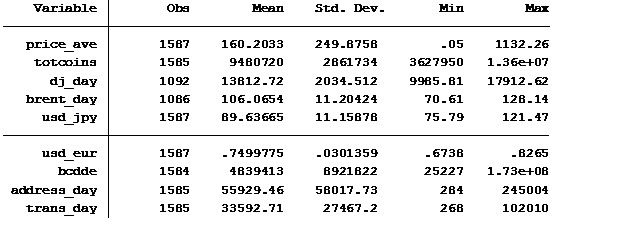
\includegraphics[width=150mm]{summary.png}

\caption{Summary Statistics}

\label{overflow}

\end{figure}

\vs

\begin{figure}[ht!]

\centering

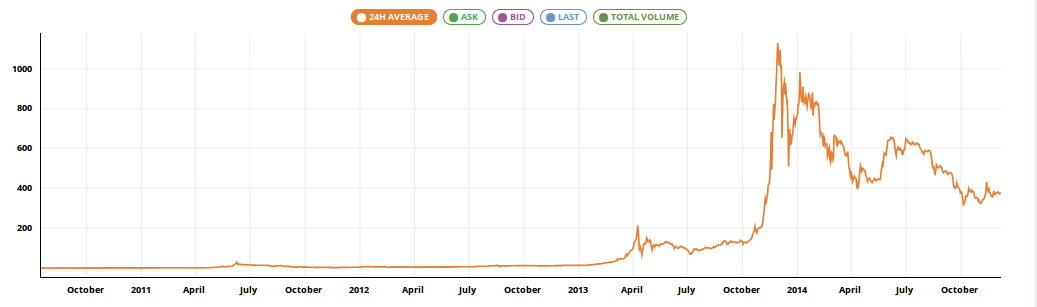
\includegraphics[width=150mm]{ave_price.png}

\caption{Bitcoin value in US Dollars}

\label{overflow}

\end{figure}

\vs

\begin{figure}[ht!]

\centering

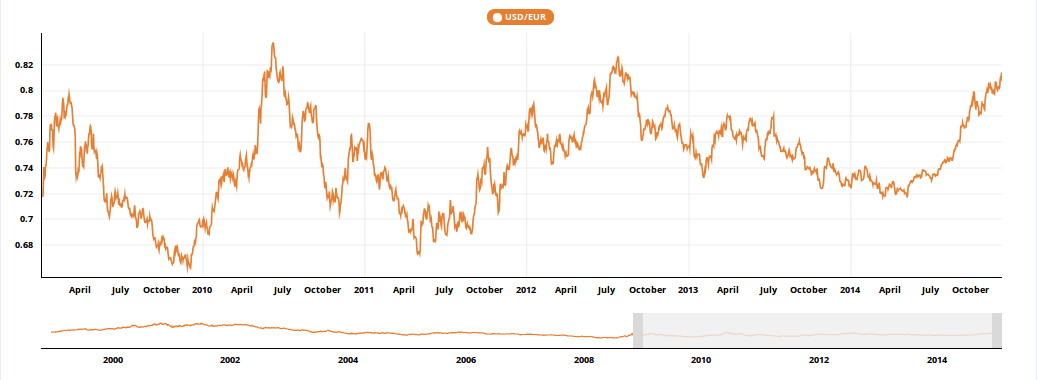
\includegraphics[width=150mm]{brent_oil.png}

\caption{Brent Oil Prices in US Dollars}

\label{overflow}

\end{figure}

\vs

\begin{figure}[ht!]

\centering

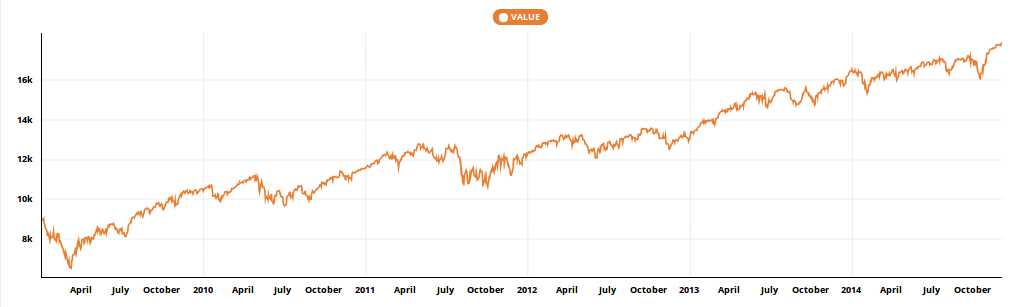
\includegraphics[width=150mm]{dj_days.png}

\caption{DOW Jones Index US Dollars}

\label{overflow}

\end{figure}

\vs

\begin{figure}[ht!]

\centering

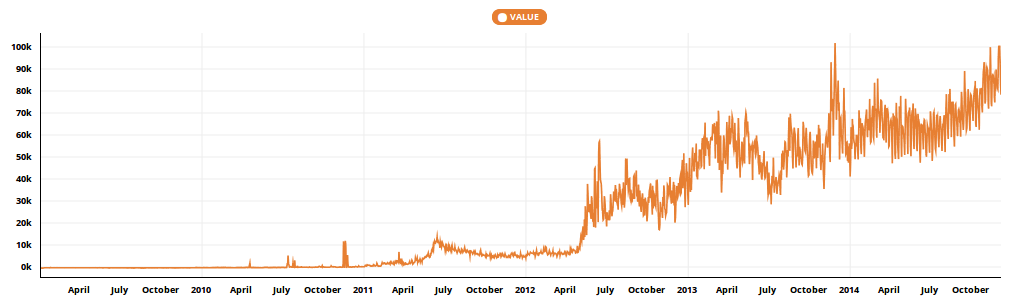
\includegraphics[width=150mm]{trans_day.png}

\caption{Number of Unique Bitcoin Transactions per Day}

\label{overflow}

\end{figure}

\vs

\begin{figure}[ht!]

\centering

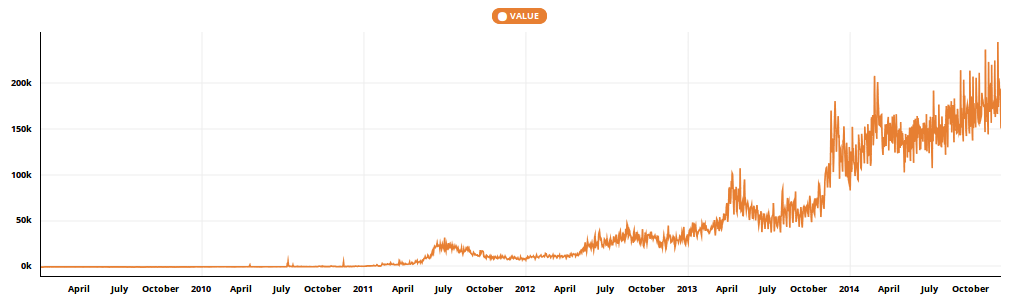
\includegraphics[width=150mm]{address_day.png}

\caption{Number of Unique Bitcoin Addresses Involved In Transactions per Day}

\label{overflow}

\end{figure}

\vs

\begin{figure}[ht!]

\centering

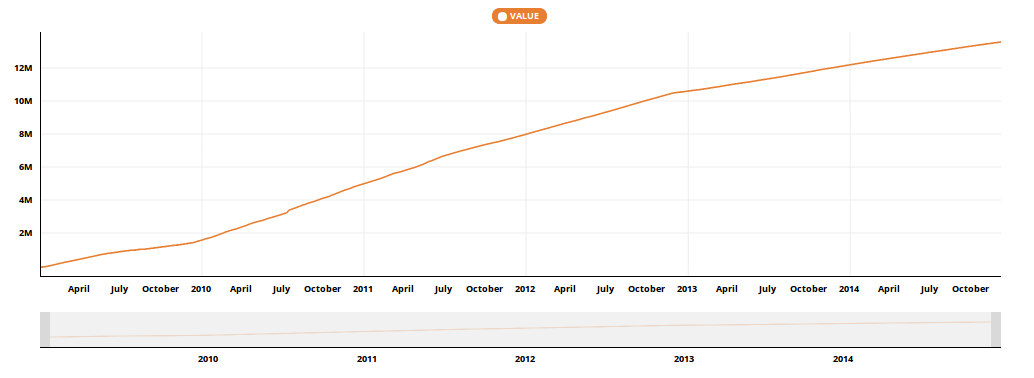
\includegraphics[width=150mm]{tot_btc.png}

\caption{Total Bitcoins}

\label{overflow}

\end{figure}

\vs

\begin{figure}[ht!]

\centering

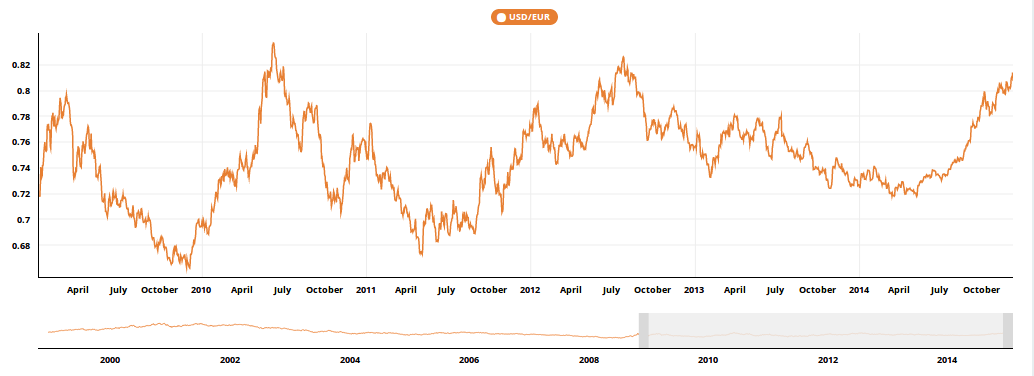
\includegraphics[width=150mm]{USD_EUR.png}

\caption{USD-EUR Exchange Rate in US Dollars}

\label{overflow}

\end{figure}

\vs

\begin{figure}[ht!]

\centering

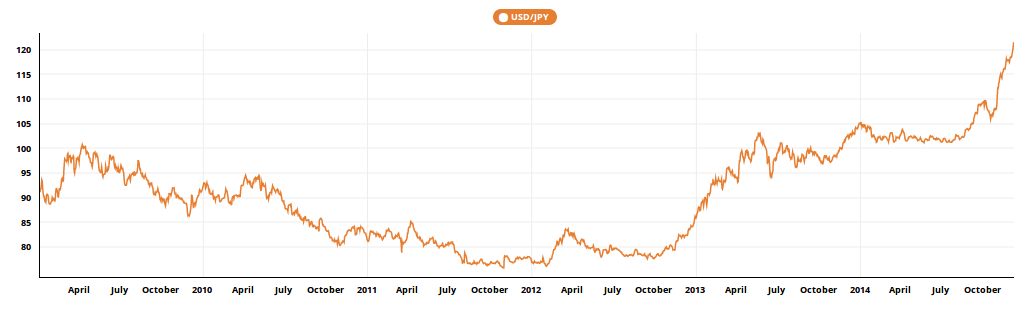
\includegraphics[width=150mm]{USD_JPY.png}

\caption{USD-JPY Exchange Rate in Japanese Yen}

\label{overflow}

\end{figure}

\clearpage

\textbf{Appendix B: Stationarity}

\vspace{5mm}

\begin{figure}[ht!]

\centering

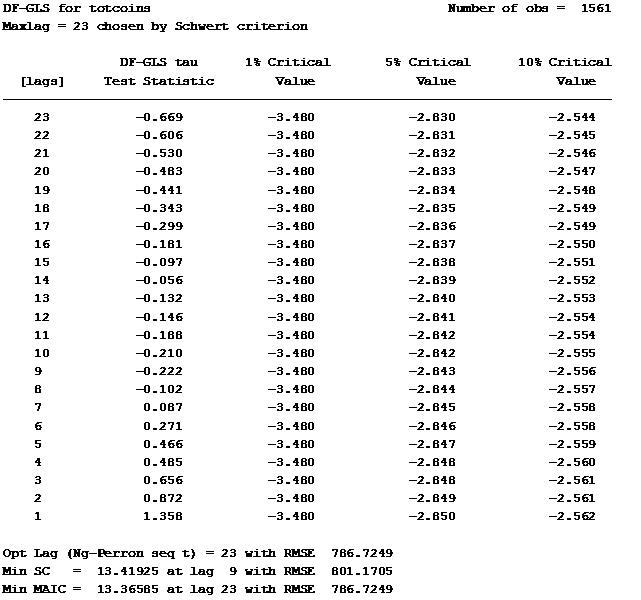
\includegraphics[width=150mm]{df_totcoins.pnon}

\label{overflow}

\end{figure}

\vspace{3mm}

\begin{figure}[ht!]

\centering

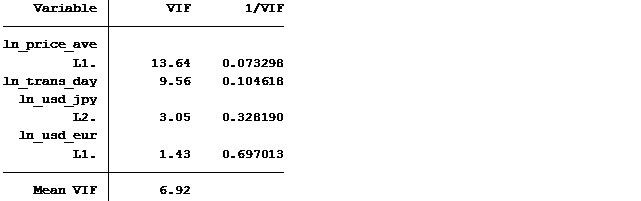
\includegraphics[width=125mm]{reg4_vif.png}

\caption{Decreased Multicolinarity}

\label{overflow}

\end{figure}

\vspace{3mm}

\begin{figure}[ht!]

\centering

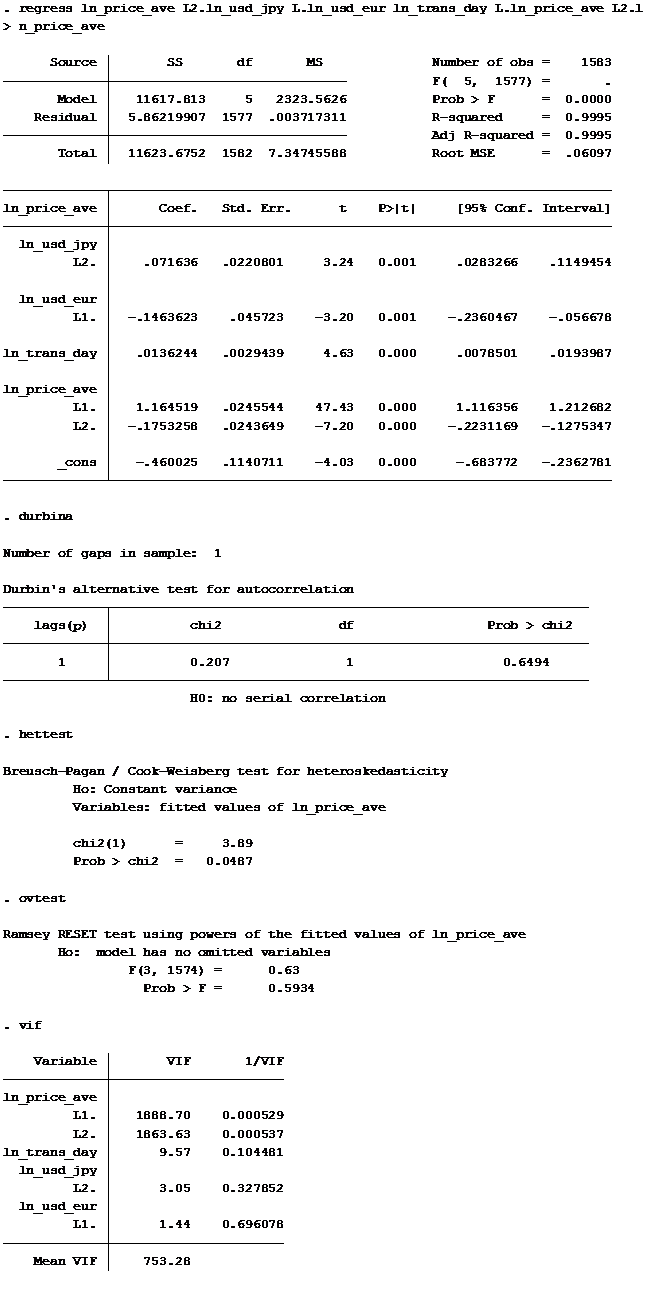
\includegraphics[width=125mm]{reg5.png}

\caption{Last Good Model}

\label{overflow}

\end{figure}

\clearpage

\newpage

\begin{figure}[ht!]

\centering

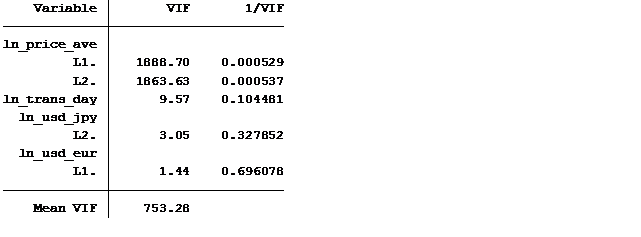
\includegraphics[width=110mm]{reg5_vif.png}

\caption{Multicolinearity of Model}

\label{overflow}

\end{figure}

\end{document}
